\documentclass{chi-ext}
% Please be sure that you have the dependencies (i.e., additional LaTeX packages) to compile this example.
% See http://personales.upv.es/luileito/chiext/

%% EXAMPLE BEGIN -- HOW TO OVERRIDE THE DEFAULT COPYRIGHT STRIP -- (July 22, 2013 - Paul Baumann)
% \copyrightinfo{Permission to make digital or hard copies of all or part of this work for personal or classroom use is granted without fee provided that copies are not made or distributed for profit or commercial advantage and that copies bear this notice and the full citation on the first page. Copyrights for components of this work owned by others than ACM must be honored. Abstracting with credit is permitted. To copy otherwise, or republish, to post on servers or to redistribute to lists, requires prior specific permission and/or a fee. Request permissions from permissions@acm.org. \\
% {\emph{CHI'14}}, April 26--May 1, 2014, Toronto, Canada. \\
% Copyright \copyright~2014 ACM ISBN/14/04...\$15.00. \\
% DOI string from ACM form confirmation}
%% EXAMPLE END -- HOW TO OVERRIDE THE DEFAULT COPYRIGHT STRIP -- (July 22, 2013 - Paul Baumann)

\copyrightinfo{\scriptsize Permission to make digital or hard copies of part or all of this work for personal or classroom use is granted without fee provided that copies are not made or distributed for profit or commercial advantage and that copies bear this notice and the full citation on the first page. Copyrights for third-party components of this work must be honored. For all other uses, contact the Owner/Author. \\
{\emph{\emph{L@S 2015}}, March 14--18, 2015, Vancouver, BC, Canada.\\
ACM 978-1-4503-3411-2/15/03. \\
http://dx.doi.org/10.1145/2724660.2728694}}
%\clubpenalty=10000 
%\widowpenalty = 10000

\title{Learner-Sourcing in an Engineering Class at Scale}

\numberofauthors{3}
% Notice how author names are alternately typesetted to appear ordered in 2-column format;
% i.e., the first 4 autors on the first column and the other 4 auhors on the second column.
% Actually, it's up to you to strictly adhere to this author notation.
\author{
\alignauthor{
        \textbf{Elena L. Glassman}\\
        \affaddr{MIT CSAIL}\\
        \affaddr{32 Vassar St.}\\
        \affaddr{Cambridge, MA 02139 USA}\\
        \email{elg@mit.edu}
}
\vfil
\alignauthor{
        \textbf{Christopher J. Terman}\\
\affaddr{MIT CSAIL}\\
        \affaddr{32 Vassar St.}\\
        \affaddr{Cambridge, MA 02139 USA}\\
        \email{cjt@mit.edu}
}
\vfil
\alignauthor{
        \textbf{Robert C. Miller}\\
\affaddr{MIT CSAIL}\\
        \affaddr{32 Vassar St.}\\
        \affaddr{Cambridge, MA 02139 USA}\\
        \email{rcm@mit.edu}
}
}

% Paper metadata (use plain text, for PDF inclusion and later re-using, if desired)
\def\plaintitle{CHI LaTeX Extended Abstracts Template}
\def\plainauthor{Luis A. Leiva}
\def\plainkeywords{Guides, instructions, author's kit, conference publications}
\def\plaingeneralterms{Documentation, Standardization}

\hypersetup{
% Your metadata go here
pdftitle={\plaintitle},
pdfauthor={\plainauthor},
pdfkeywords={\plainkeywords},
pdfsubject={\plaingeneralterms},
% Quick access to color overriding:
%citecolor=black,
%linkcolor=black,
%menucolor=black,
%urlcolor=black,
}

\usepackage{graphicx} % for EPS use the graphics package instead
\usepackage{balance} % useful for balancing the last columns
\usepackage{bibspacing} % save vertical space in references

\usepackage{tabularx}

\begin{document}

\maketitle

\begin{abstract}
Teaching computer architecture as a hands-on engineering course to approximately 250 MIT students per semester requires a large, dedicated teaching staff. This Spring, a shortened version of the course will be deployed on edX to a potentially far larger cohort of students, without additional teaching staff. To better support students, we have deployed developmental versions of three learner-sourcing systems to as many as 500 students. These systems harvest and organize students' collective knowledge about debugging and optimizing solutions. We plan to deploy and study the next iteration of these systems on edX this Spring.
\end{abstract}

%\category{H.5.m}{Information interfaces and presentation (e.g., HCI)}{Miscellaneous}.
%See \cite{ACMCCS}
%See: \url{http://www.acm.org/about/class/1998/}
%for help using the ACM Classification system.
%\textcolor{red}{Optional section to be included in your final version, but strongly encouraged.}


% =============================================================================
\section{Introduction}
% =============================================================================
One-on-one tutoring has been established as a costly gold standard in education \cite{Bloom}. In MOOCs, the teacher-to-student ratio is drastically lower. Teaching staff cannot walk around the lab to get a sense of common success and failures. They also suffer from the ``curse of knowledge'': the difficulty experts have when trying to see something from a novice's point of view \cite{curse}.

We are developing systems that harvest and organize students' collective knowledge about debugging and optimizing solutions. Students themselves are each becoming experts on their own bugs and solutions. The key design principle is that students write hints immediately after completing a task or fixing a bug. Later, other students can use these hints to help guide them to a correct solution or better design. While students do not have the pedagogical content knowledge to necessarily generate optimal explanations, they also do not suffer from the curse of knowledge. These systems relieve some of the pressure on the relatively small teaching staff, and give students the valuable educational experiences of reflection and generating explanations \cite{selfexplanation}. 
%\begin{figure}[!h]
%\centering
%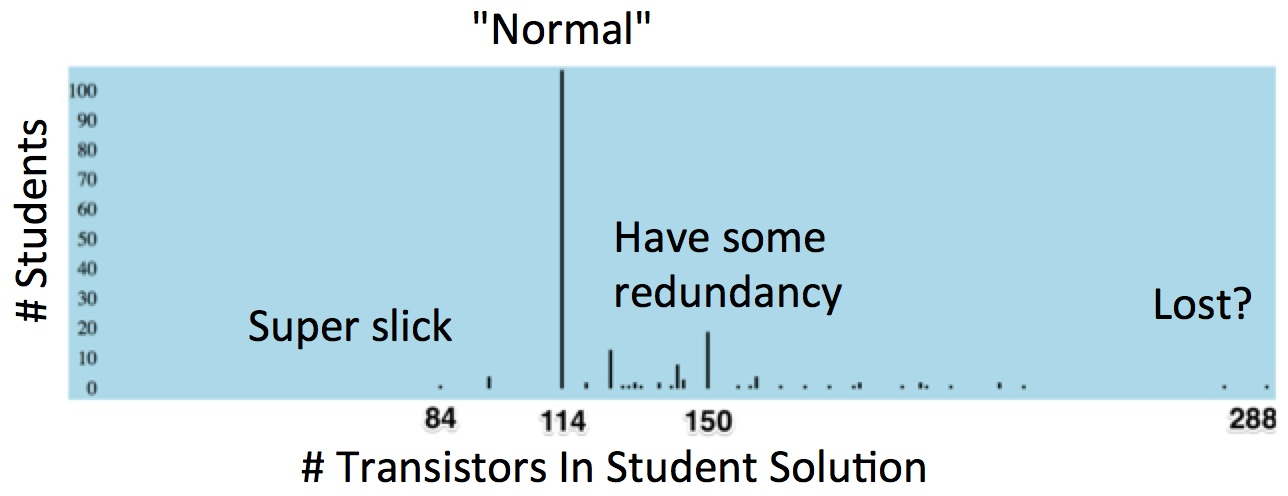
\includegraphics[width=0.9\columnwidth]{distributionOfTransistors.jpg}
%\caption{Distribution of the students' correct solutions (Full Adders), as a function of the %number of transistors.}
%\label{fig:figure1}
%\end{figure}

We present ongoing case studies of three systems deployed in an undergraduate computer architecture course at MIT. Around 250 students enroll each semester. The three deployed systems have distinct objectives: (1) learner-source hints for debugging, (2) learner-source hints for optimization, and (3) prompt students to reflect on other students' solutions. Learner-sourcing refers to crowd-sourcing within the community of students enrolled in a course.

These systems have already been deployed at scale to as many as five hundred students over multiple semesters. Our case studies prepare us to design, deploy, and study the next iteration of these systems on edX this Spring. Throughout the process, we continue to develop design principles that can guide future learner-sourcing systems for engineering classes.

\section{Related Work}

In order to generate hints for others, students must reflect on their bug, solution, or optimization, and then explain. We review relevant literature at the intersection of learning theory and engineering education.

\subsection{Reflection}
Reflection and confusion are both treated at length in learning theory literature. Piaget theorized that cognitive disequilibrium, experienced as confusion, could trigger learning: the creation or restructuring of knowledge schema \cite{disequilibrium}. However, D'Mello et al. point out that, for this learning to take place, it is important for confusion to be both appropriately injected and resolved \cite{productiveconfusion}. Dewey theorized that reflection is a critical method for triggering that transformation from conflict and doubt into clarity and coherence \cite{dewey1933}. Turning that reflection into a self-explanation also improves understanding \cite{selfexplanation}. Turns et al. \cite{asee} argue that the absence of reflection in traditional engineering education scholarship is a significant gap. In this work, we aim to design scalable automated opportunities for students to reflect in an engineering course.
\subsection{Peer Instruction and Assessment}
While reflection is valuable in its own right, it is also a building block of larger frameworks, like Peer Instruction \cite{mazur} and Peer Assessment \cite{peerassessment}. Reflecting on a peer's conceptual development or alternative solution may bring about cognitive conflict that prompts reevaluation of the student's own beliefs and understanding \cite{kavanagh}. We aim to trigger productive cognitive conflict that students can attempt to resolve through written reflection.
\subsection{Generating Hints for Students}
With a mixture of automation and human input, helpful hints have been delivered to students in multiple problem domains. HelpMeOut \cite{helpmeout} tracks the changes programmers make when fixing a compilation error or runtime exception. Users can write helpful messages to accompany these automatically extracted bug fixes. Our work uses a similar strategy for learner-sourcing hints for a new domain. We also learner-source optimization advice.

\section{Debugging} %: crowd-sourcing hints from learners}                                                
In our course, students design entire simulated processors composed of logic gates. These processors can be challenging to debug even with the one­-on-­one help of seasoned teaching staff. Students who have recently resolved a particular bug can be in a better position than available staff members to help a fellow student with the same bug. Bugs are revealed by verification failures found by a staff-designed testbed. There are hundreds of possible unique verification failures. The course forum's generic structure does not lend itself to searching for other students' difficulties with particular verification failures. 

%\begin{figure*}
%\centering
%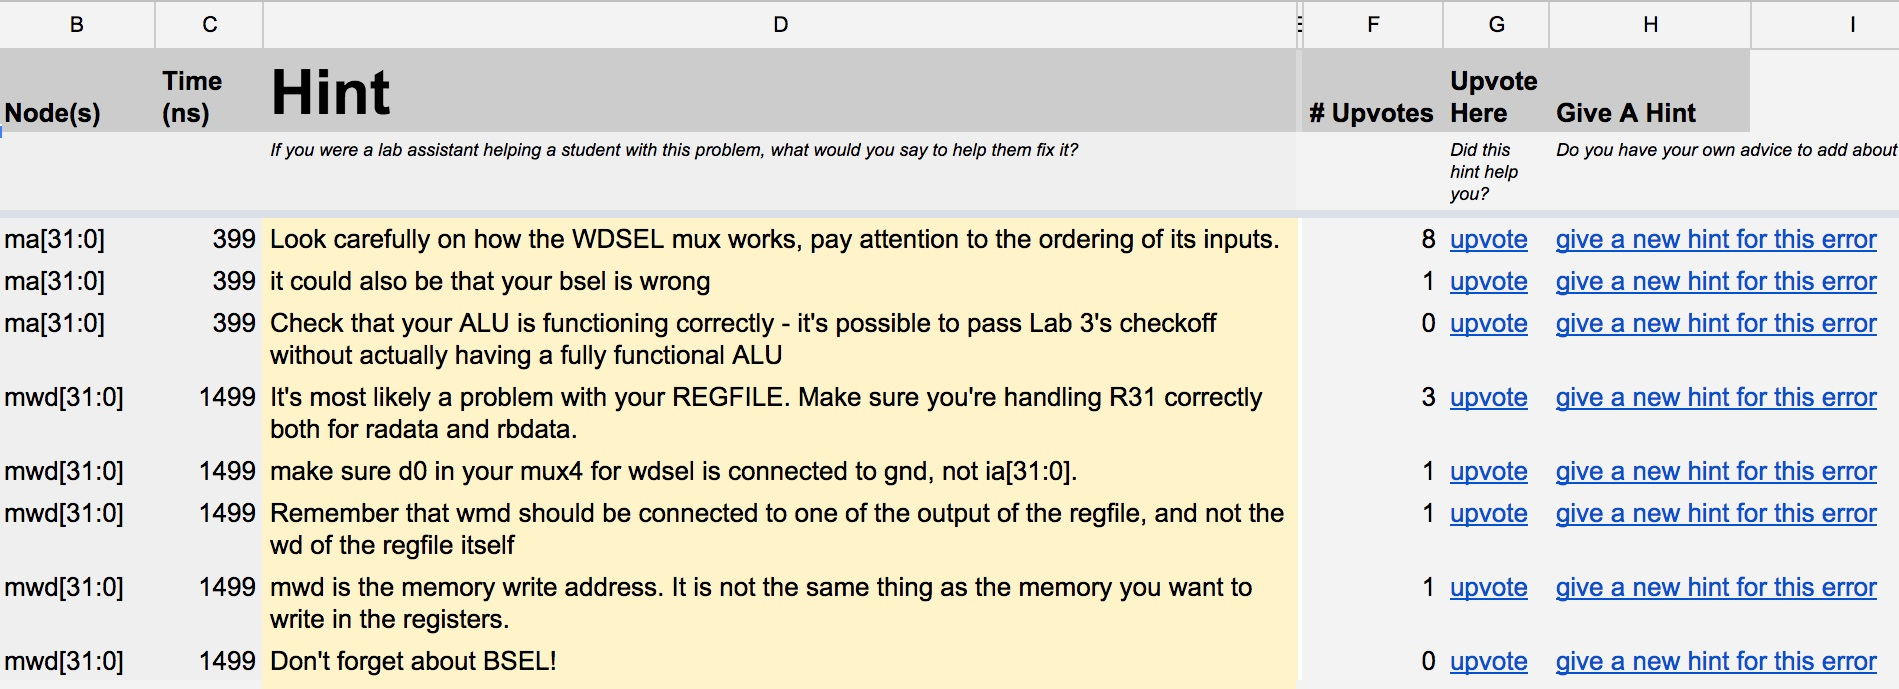
\includegraphics[width=0.75\textwidth]{DearBeta.jpg}
%\caption{{\it Dear Beta} serves as a central repository of debugging advice for and by students, indexed by verification failures. For example, there are three separate crowd-sourced hints for the first verification failure ($ma[31:0], 399ns$), ordered from greatest to least upvotes. The left two columns, wire name and time, uniquely characterize the verification failure. The central pale yellow column is for the hint. The right-most three columns display the number of upvotes, a link that will add an upvote to the hint, and a link to add a different hint for the same verification error. {\it Dear Beta} is implemented with Google Spreadsheets, Forms, and Apps Scripts.}
%\label{fig:figure3}
%\end{figure*}

We built {\it Dear Beta}, a system that serves as a central repository of debugging advice for and by students, indexed according to verification failures. As soon as a student resolves a bug, they can post an explanation of their bug on Dear Beta along with the verification failure it caused. Students can easily look up advice for their particular failure. Students upvote hints they found helpful. Initial evidence suggests it was consistently helpful. One teaching assistant said, ``Whenever I went to help a student, I first asked them if they'd checked Dear Beta.'' We will create a Meteor or Django-backed version for edX students this Spring. 

\marginpar{
\begin{figure}
\centering
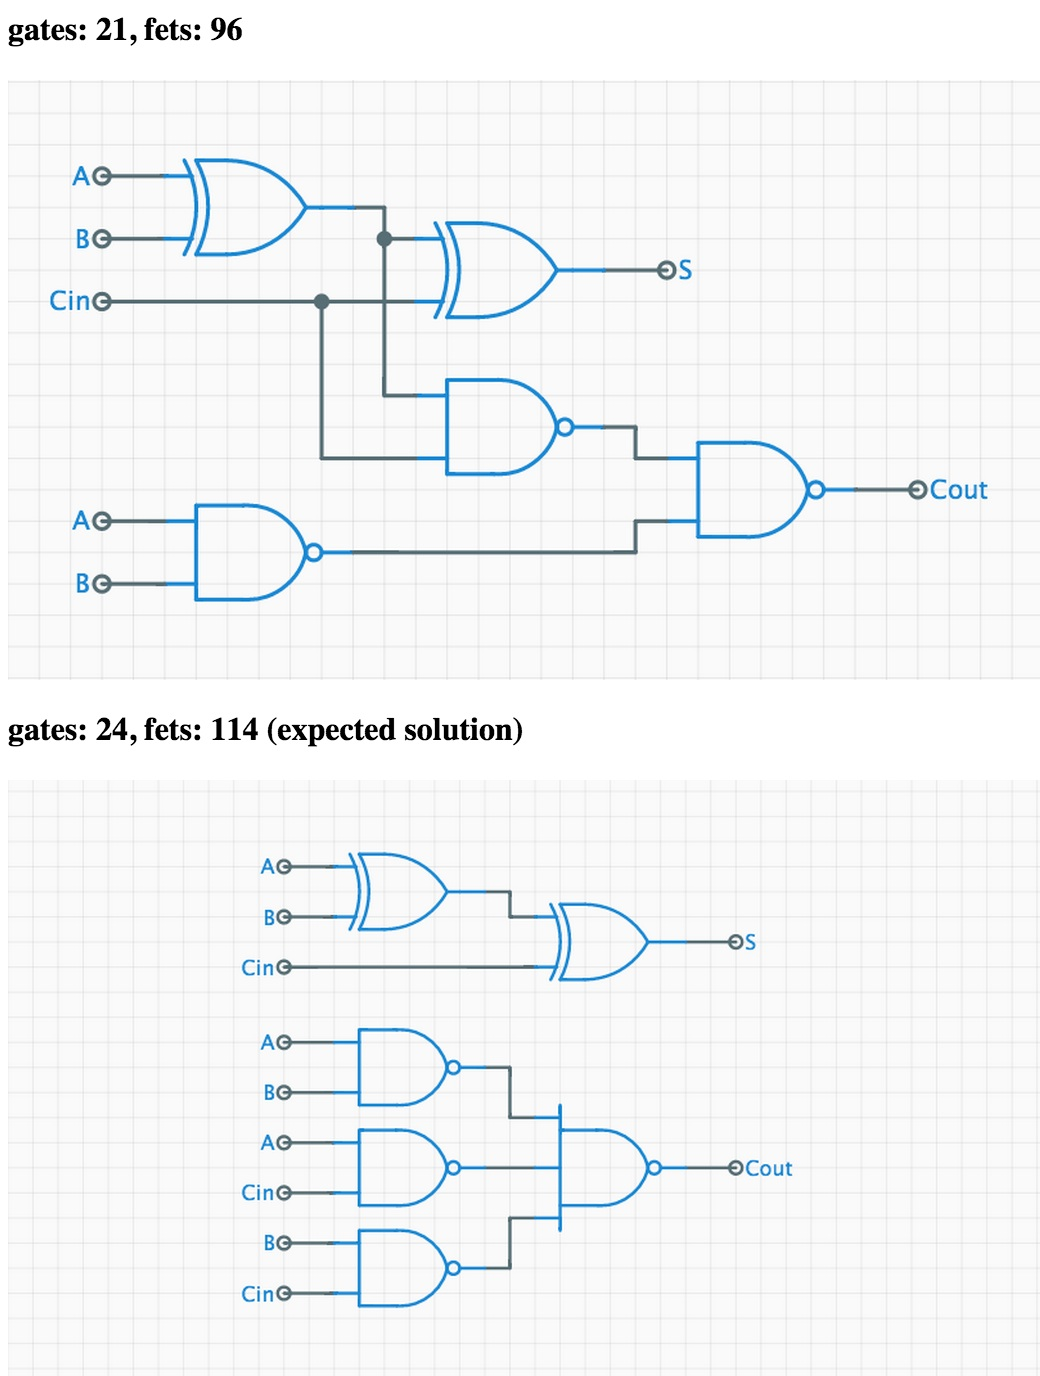
\includegraphics[width=1.0\marginparwidth]{solutionComparison.jpg}
\caption{Two correct student solutions (Full Adders), composed of different numbers and arrangements of XOR and NAND gates. The more optimal solution has only 21 gates and 96 transistors (FETs) while the expected, less optimal solution has 24 gates and 114 transistors.}
\label{fig:figure2}
\end{figure}
}

\section{Optimization}%: crowd-sourcing hints and results from learners}

Students optimize their own processors for additional points, which are a function of the processor's size and speed. Students also get a long list of optimization hints written by staff that students consult when choosing which optimizations to implement. Students can take hours to act on a single optimization hint, without knowing which has the greatest payoff.


We deployed a system for learner-sourcing optimization hints and results, with the aim of giving students more transparency and assistance. We indexed hints according to whether they were intended to reduce the processor's size, increase its speed, or both. We also gave students the option of submitting the magnitude of the speed and size improvement they got from acting on a hint, so that future students could gauge which optimization hints were most beneficial on average. 

This system was not as successful as Dear Beta. We are, however, confident that students are ultimately capable of generating high-quality processor optimization hints, based on results shown in the next section on reflection and comparison.

\section{Reflection}%: Prompted Reflections on Other Students' Solutions}

Early on in our course, students design a piece of their processor: a working Full Adder. Students create a variety of solutions that fit the behavior specification. Some are unnecessarily large, and some optimize to use as few transistors as possible. In this scenario, fewer transistors translate to better performance.

%\begin{figure}[!h]
%\centering
%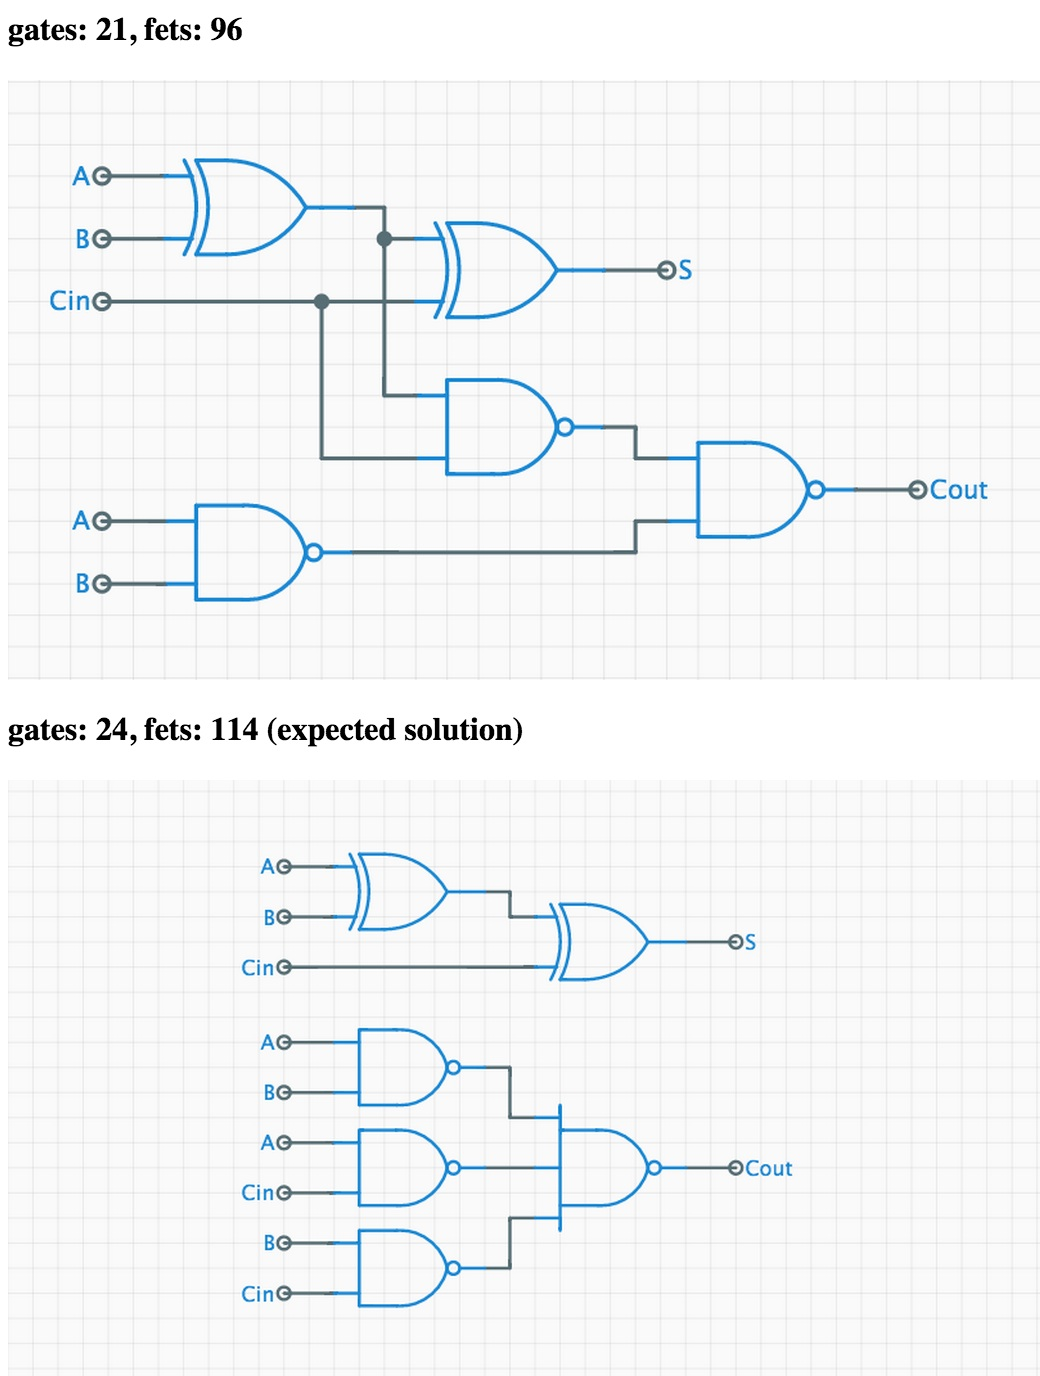
\includegraphics[width=1.0\columnwidth]{solutionComparison.jpg}
%\caption{Two correct student solutions (Full Adders), composed of different numbers and arrangements of XOR and NAND gates. The more optimal solution has only 21 gates and 96 transistors (FETs) while the less optimal solution has 24 gates and 114 transistors.}
%\label{fig:figure2}
%\end{figure}


Through exploration of hundreds of previous students' solutions, we picked a representative set. Each student was then shown their own solution next to (1) a worse solution in the representative set and (2) the best solution in the representative set. Students were asked to give a hint to future students about how to improve the poorer solution in each pairing (see Figure \ref{fig:figure2}). When the student's own solution is the better solution in the pair, then the student can hint at what the peer had conceptually missed. For example, {\it Remember DeMorgan's Law: you could replace the `OR' of `ANDs' with a `NAND' of `NANDs.'} When the students' own solution is the poorer solution in the pair, they are challenged to first understand how the better solution uses fewer transistors and then write a hint about the insight for a peer.

\marginpar{
\begin{table}
\begin{tabularx}{\marginparwidth}{ |X| }
\hline
{\bf Learner-sourced Advice} \\
    \hline
    ``Do not try to be too clever with $C_{out}$---design your schematic as the expression is written. This way you will achieve the [standard] schematic.'' \\ \hline
``Mutate the boolean function for $C_{out}$ such that all OR and AND operations are being NOT'ed. This allows you to design a circuit using only naturally inverting CMOS gates.'' \\ \hline 
``I would ask: is there a way for you to use some intermediate node in one circuit to bypass a CMOS gate in the other, leading to a reduction of used mosfets?'' \\ \hline
    \end{tabularx}
\caption{Examples of learner-sourced advice for optimizing fellow students' Full Adders.}
\label{tab}
\end{table}
}

This reflection and explanation process is pedagogically valuable on its own. In addition, students' explanations give a rich window into their understanding, while serving as strikingly cogent potential advice to future students (see Table \ref{tab}). The online version of this course may afford us the opportunity to deliver these optimization hints back to students.

\section{Conclusions and Future Work}

This work in progress is the accumulation of several semesters of system development and deployment in a large undergraduate engineering course. Students can write high-quality optimization advice when their solution is paired with a distinct peer solution. Learner-sourced debugging hints, indexed by verification failures, are a valuable student resource. We are preparing to deploy the next iteration of these systems on edX this Spring, while considering how best to measure impact on the student learning experience.

\section{Acknowledgments}

We appreciate the support of the NSF Graduate Research Fellowship, Quanta Computer, and the Amar Bose Teaching Fellowship for funding this work.



\bibliographystyle{acm-sigchi}
\bibliography{learnersourcing}
\balance
\end{document}

A Full Adder adds two bits of information, plus an optional `carry-in' bit, to produce a `sum' bit and `carry out' bit.
Some of these domains can be solved by students taking one of a family of sequential steps toward the final correct answer, such as logic proofs and physics problems. Other domains are less constrained, e.g., introductory programming assignments. Finally, s

Some domains are complex enough that hints are based on errors and local information about a student's work, rather than a global understanding of that students' work. Our students' processors are complex enough that they fall into this third, most complex problem domain.

 We are still diagnosing why. 
